\documentclass[12pt,a4paper]{scrartcl}
\usepackage[utf8]{inputenc}
\usepackage[T1]{fontenc}
\usepackage[french]{babel}
\usepackage{textcomp}
\usepackage{amsmath,amssymb}
\usepackage{lmodern}
\usepackage{graphicx}
\usepackage[dvipsnames,svgnames]{xcolor}
\usepackage{microtype}
\usepackage{hyperref}
\usepackage{lipsum}
\usepackage[pointedenum]{paralist}
\usepackage{listings}
\usepackage{graphicx}
\usepackage{multicol}
\usepackage{xspace}
\usepackage{xcolor}
\usepackage{amsthm}
\usepackage{tikz}
\usepackage{scrlayer-scrpage}

\bibliographystyle{plain}

\ihead{Fabio DAUSSY, Théorie des Graphes}
\ohead{Initiation à LATEX}

\lstset{
language=c,
backgroundcolor=\color{Grey!10},
keywordstyle=\color{DarkBlue}\bfseries,
tabsize=4,
}

\hypersetup{colorlinks=true,linkcolor=Brown,breaklinks=true,pdfstartview=XYZ}
\frenchsetup{StandardItemLabels=true}

\newcommand{\G}{Soit $G(X,U)$, un graphe d'ordre $n$} %commande simple
\newcommand{\coul}[2]{\color{#1} #2 \color{black}} %commande avec paramêtres

\title{La Théorie des graphes}
\author{Fabio Daussy}
\date{\today}

\theoremstyle{plain}
	\newtheorem{theoreme}{Théorème}[section]
	\newtheorem{proposition}[theoreme]{Proposition}
	\newtheorem{corollaire}[theoreme]{Corollaire}
	\newtheorem{definition}[theoreme]{Définition}
	\newtheorem{exo}{Exercice}

\theoremstyle{remark}
	\newtheorem*{exemple}{Exemple}
	\newtheorem*{remarque}{Remarque}

\begin{document}
\maketitle

\begin{abstract}
Dans ce cours texte, nous allons voir brievement des éléments essentiels de la théorie des graphes. Inspiré du cours de Philippe Langevin.
Notamment sa définition et jusqu'où le sujet peut s'étendre.
Vous devez probablement connaître ce fameux jeu où l'on vous demande de dessiner une maison sans lever le crayon. Ce même problême est aussi connu sous la forme du problême des ponts et des îles. C'est un problême type de la théorie des graphes qui a été résolu par Euler\footnote{Leonhard Euler (1707-1783) est un mathématicien et physicien suisse qui a fait de nombreuses découvertes en théorie des graphes et en calcul infinitésimal. Source : Wikipédia}.
\end{abstract}

\tableofcontents

\section{Introduction}
"La théorie des graphes s’est développée au cours du XX$^e$ siècle,
Las Vergnas nous rappelle que terminologie de graphe a été
introduite par Sylvester en 1877, et que le premier livre sur la théorie
des graphes a été écrit par D.König en 1936. La génèse de la théorie
des graphes semble être une étude de Léonard Euler, un très célèbre
mathématicien du XVIII$^e$ siècle. Dans un article publié en 1736, il traite
un problème devenu classique, illustré par la devinette : peut-on faire
une promenade passant une fois par chacun des sept ponts de la ville
de Koenigsberg (\ref{g.koen}) ? Il suffit de faire quelques essais pour se convaincre
de l’impossibilité de réaliser une telle promenade. L’objectif de cette
section est de dégager un résultat général."\footnote{Introduction du cours sur la théorie des graphes de Monsieur Philippe Langevin \cite{TAG}}

\begin{figure}
	\centering
	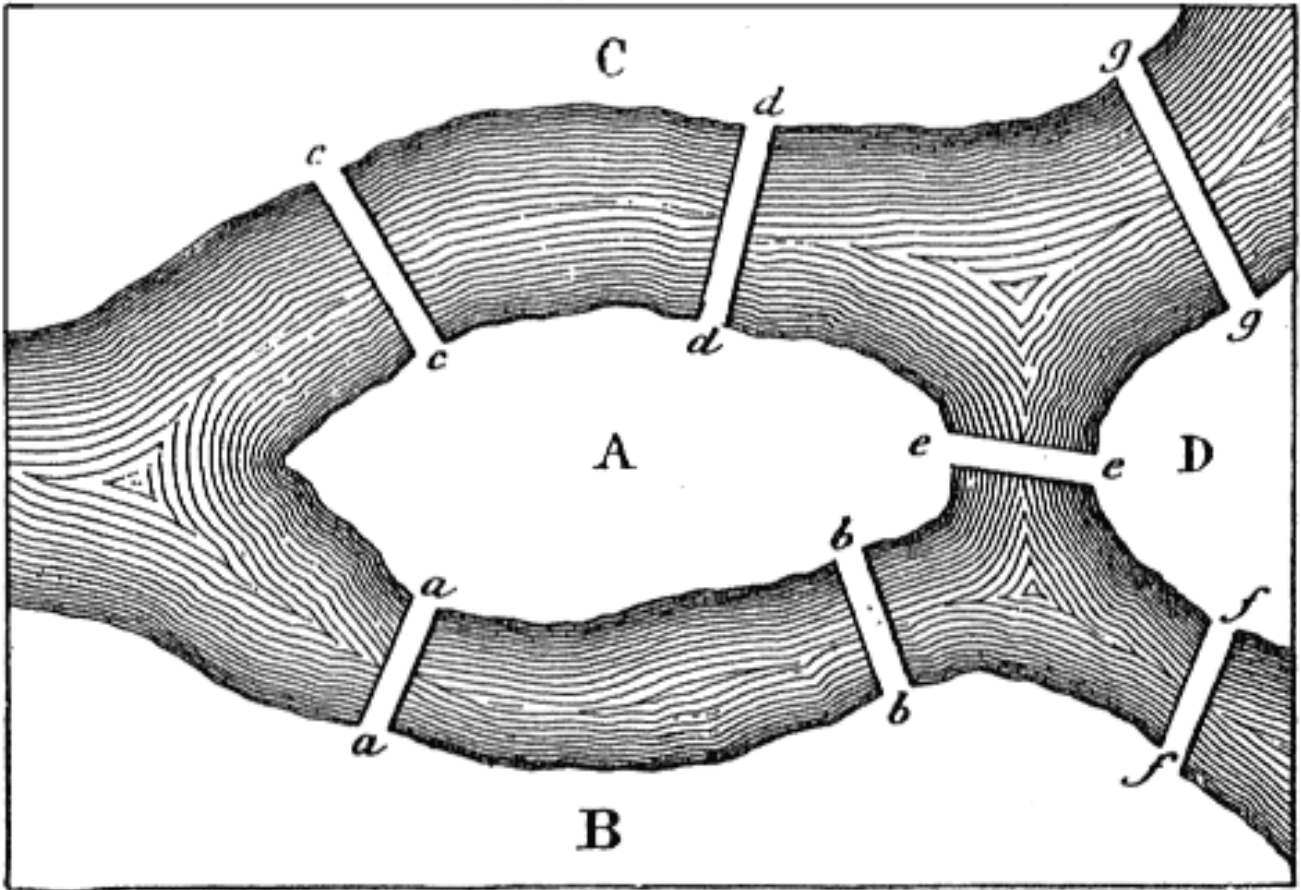
\includegraphics[scale=0.25]{pontsiles.png}
	\caption{Les ponts de Koenigsberg en 1759}\label{g.koen}
\end{figure}

\section{Notion de bases}

\begin{definition}
Un graphe $G$ est un couple $(X,U)$, où $X$ est un ensemble de \textbf{sommets} et
$U$ un sous-ensemble tel que $U \subseteq \mathcal{P}_2(X)$, ce sont les \textbf{arêtes} du graphe 
\end{definition}

\begin{exemple}
	Ainsi, pour le graphe maison G en figure \ref{g.maison} nous avons :
\[X:= \{ 1,2,3,4,5 \}\quad
U:= \{ \{1,2\},\{1,3\},\{3,4\},\{2,4\},\{2,5\},\{4,5\},\{2,3\},\{1,4\} \}\]	
\end{exemple}

\begin{definition}
	On dit que deux sommets $x,y \in X$ sont \textbf{adjacents} si et seulement si $\{x,y\} \in U$.
\end{definition}

\begin{definition}
	Soit un sommet $s$. On appelle \textbf{degré} de $s$ le nombre d'arêtes qui sont \textbf{incidentes} en $s$. Le degré d'un sommet $s \in X$ se note aussi $deg(s)$.
\end{definition}

\begin{exemple}
	L'ensemble des degrés des sommets de $G$ (\ref{t.deg}).
\end{exemple}

\begin{table}[tbp]
	\centering
	\begin{tabular}{|l|l|l|l|l|l|}
	\hline
	sommet & 1 & 2 & 3 & 4 & 5 \\
	\hline
	degré  & 3 & 4 & 3 & 4 & 2 \\
	\hline
	\end{tabular}
	\caption{L'ensemble des degrés des sommets du graphe $G$ (\ref{g.maison})}\label{t.deg}
	\end{table}

\begin{proposition}
	Soit $m$ le nombre d'arêtes du graphe,
	\begin{equation}
		\sum_{s \in X} \text{deg}(s)\quad=\quad 2\times m
	\end{equation}\label{eq.degsum}
		
\end{proposition}

\begin{definition}
	On appelle l'\textbf{ordre} d'un graphe $G$ le nombre de sommets qui le composent (i.e. le cardinal de $X$).
\end{definition}

\begin{definition}
	Un sommet $s$ est dit \textbf{isolé} si et seulement si son degré vaut $0$.
\end{definition}

\begin{definition}
	Soit $n$ l'ordre du graphe. Un sommet $s$ est dit \textbf{dominant} si et seulement si son degré vaut $n-1$.
\end{definition}

\begin{definition}
	Si tous les sommets d'un graphe d'ordre $n$ sont dominants
alors on appelera ce graphe, le \textbf{graphe complet} d'ordre $n$. On le note $\mathbb{K}_{n}$.
\end{definition}

\begin{figure} % flottant
	\centering
	\begin{tikzpicture}[scale=.9,auto=center,every node/.style={circle,fill=red!20}]
  	\node (a1) at (0,0) {1};
  	\node (a2) at (0,4) {2};
  	\node (a3) at (4,0) {3};
  	\node (a4) at (4,4) {4};
  	\node (a5) at (2,6) {5};
  	
  
  	\draw (a1) -- (a2);
  	\draw (a1) -- (a3);
  	\draw (a2) -- (a4);
  	\draw (a4) -- (a3);
  	\draw (a2) -- (a5);
  	\draw (a4) -- (a5);
  	\draw (a2) -- (a3);
  	\draw (a4) -- (a1);
	\end{tikzpicture}
	\caption{Le graphe maison $G(X,U)$ }\label{g.maison}
\end{figure}


\section{Connexité}

\begin{definition}
	Soit $G(X,U)$ un graphe d'ordre $n$, on appelle \textbf{chemin} toute suite de sommets 
	\[
	x_1,x_2,\dots,x_l\quad \forall x_i \in X,\ i \in [1,n] \qquad \text{tel que deux sommets consécutifs sont adjacents}
	\]
\end{definition}

\begin{remarque}
	Un chemin dont les extrémités sont le même sommet est un \textbf{cycle}.
\end{remarque}
Notons que:
	\begin{itemize}
		\item $l$ est la \textbf{longueur} du chemin.
		\item $x_1$ et $x_l$ sont les \textbf{extrémités} du 				chemin.
	\end{itemize}

\begin{definition}
	On dit que deux sommets $x,y$ sont \textbf{liés} si et seulement si, il existe un chemin d'extrémités $x$ et $y$. On note la liaison:
	\[
	x \leadsto y	
	\]
\end{definition}

\begin{proposition}
	La relation de liaison entre deux sommets est une \textbf{relation d'équivalence}. Les classes d'équivalences de cette relation sont appelées \textbf{composantes connexes}.
\end{proposition}

\begin{exemple}
 Le graphe (\ref{g.compconn}) possède 2 composantes connexes
\end{exemple}

\begin{figure}
	\centering
	\begin{tikzpicture}[scale=.9,auto=center,every node/.style={circle,fill=blue!20}]
  	\node (a1) at (1,1) {1};
  	\node (a2) at (0,2) {2};
  	\node (a3) at (4,0) {3};
  	\node (a4) at (3,3) {4};
  	\node (a5) at (2,5) {5};

	\draw (a1) -- (a3);
	\draw  (a2) -- (a4);
	\draw (a5) -- (a4);
	\draw (a5) -- (a2);
  	
  	\end{tikzpicture}
	\caption{Un graphe d'ordre 5}\label{g.compconn}
\end{figure}

\begin{remarque}
	On appelle \textbf{graphes connexes} les graphes à une composante connexe.
\end{remarque}

\section{Graphe Eulerien}\label{euler}

\begin{definition}
	 Un chemin \textbf{eulérien} dans un graphe est un chemin qui passe par toutes les arêtes du graphe une et une seule fois
\end{definition}

Le théorème d'Euler (\ref{th.euler}) permet de vérifier s'il existe ou non un cycle Eulérien dans le graphe maison (\ref{g.maison})

\begin{theoreme}\label{th.euler}
	\G, sans point isolé, possède un \textbf{cycle eulérien } si et seulement si:
	\begin{enumerate}
	\item Le graphe est \textbf{connexe}
	\item Tous les degrés des sommets sont \textbf{pairs}
	\end{enumerate}
\end{theoreme}

Le graphe maison (\ref{g.maison}) est bien connexe. En revanche, le sommet 1 est de degré impair donc il n'est pas eulérien. 
Démontrons ce théorême :
\begin{proof}
	\G, dont tous les sommets sont de degré pair. On choisit un sommet $x_0$. On construit un chemin de proche en proche en s'interdisant de repasser deux fois pas la même arête tant que possible. Cette promenade s'arrête en $x_0$ (point de départ).
	On considère le graphe partiel composé des arêtes restantes, il n'est pas forcément connexe. Chaque composante connexe est un graphe d'ordre $< n$ car $x_0$ est isolé. Les parités des degrés restent inchangées donc chaque composante connexe admet un \textbf{cycle eulérien}. On dit que chaque composante connexe du graphe partiel possède un représentant sur la promenade.
	
Ainsi pour faire le cycle, il suffit de passer sur la promenade initial, et à chaque représentant, on trace son cycle eulérien jusqu'à $x_0$ et le cycle eulérien sur le graphe initial est effectué.
\end{proof}

\begin{exemple}
Dans le graphe \ref{g.eulerien}, le sommet \coul{red}{2} joue le rôle de $x_0$.
La promenade est dessinée en \coul{blue}{bleu} et le cycle eulérien du graphe partiel sans la promenade est dessiné en \coul{yellow}{jaune}.
 Ainsi, pour tracer sans "lever le stylo" ce cycle eulérien, on part de 2, on suit la promenade \coul{blue}{bleue}. Une fois arrivé au sommet \coul{purple}{1}
\marginpar{1 est représentant de la promenade}
, on réalise le cycle jaune, puis on boucle le cycle en sur 2.
\end{exemple}

	\begin{figure}
	\centering
		\begin{tikzpicture}
		\node[shape=circle, fill=purple!50] (a1) at (0,0) {1};
		\node[shape=circle, fill=red!50] (a2) at (2,-2) {2};
		\node[shape=circle, fill=green!50] (a3) at (4,0) {3};
		\node[shape=circle, fill=green!50] (a4) at (4,4) {4};
		\node[shape=circle, fill=green!50] (a5) at (2,6) {5};
		\node[shape=circle, fill=green!50] (a6) at (0,4) {6};

		\draw [draw=blue] (a1) -- (a2);
		\draw [draw=blue] (a2) -- (a3);
		\draw [draw=blue] (a3) -- (a4);
		\draw [draw=blue] (a4) -- (a5);
		\draw [draw=blue] (a5) -- (a6);
		\draw [draw=blue] (a6) -- (a1);
		
		\draw [draw=yellow] (a1) -- (a3);
		\draw [draw=yellow] (a6) -- (a3);
		\draw [draw=yellow] (a4) -- (a1);
		\draw [draw=yellow] (a6) -- (a4);				
		
		\end{tikzpicture}
	\caption{Graphe eulérien d'ordre 6}\label{g.eulerien}
	\end{figure}

\section{Implantation en langage C}

Nous allons implanter les graphes en langage C. Pour cela nous allons utiliser la structure de données suivante (\ref{c.graphe}).


\lstinputlisting{graphe.h}\label{c.graphe}
\textit{nbs} correspond au nombre de sommet du graphe de le structure. \textit{mat} est une matrice de booléen de taille  nbs $\times$ nbs. Chaque sommet est représenté par un nombre $<$ nbs. Ainsi, si vous souhaitez accéder à l'arête entre le sommet 1 et 3; il suffit de chercher dans la matrice soit \textbf{mat[1][3]}, soit \textbf{mat[3][1]}. S'il y a une arête entre le sommet 1 et 3 alors \textbf{mat[1][3]} vaut 1. 0 sinon. \textit{clr} est un tableau de taille nbs qui va simplement permettre de se repérer lors d'un parcours du graphe. On colorie les sommets qu'on a parcouru pour ne plus retourner dessus plus tard dans l'algorithme. Il sert de condition d'arrêt.
On peut alors en déduire un algorithme de décision pour savoir si un graphe est eulérien ou non. Le code se trouve ici (\ref{c.eulerien})

\lstinputlisting{eulerien.c}\label{c.eulerien}

La complexité de cet algorithme est quadratique, il est en $O(n^2)$ si on considère que $n$ est la taille l'ordre du graphe passé en paramêtre.

\section{Conclusion}

Nous n'avons qu'effleuré le sujet immense que sont les graphes, ceux-ci sont partout autour de nous. Mais l'intêret de cette courte initiation était de vous donner une petite soif de savoir sur les graphes. En espérant que j'ai, au moins partiellement, réussi à vous transmettre cette envie.

\bibliography{graphe}

\end{document}
